\documentclass{standalone}
\usepackage[T1]{fontenc}
\usepackage[utf8]{inputenc}          % needed for French accents
\usepackage{pgfplotstable}
\usepackage{pgfplots}
\pgfplotsset{compat=1.18}
\usepackage{siunitx}                 % optional, nicer y‑axis numbers
\usepackage{booktabs}                % pretty tables for the optional preview

% -------------------------------------------------
% Helper that removes the internal \pgfpl@@ wrapper
% -------------------------------------------------

\begin{document}
% This file was created with matplot2tikz v0.4.0.
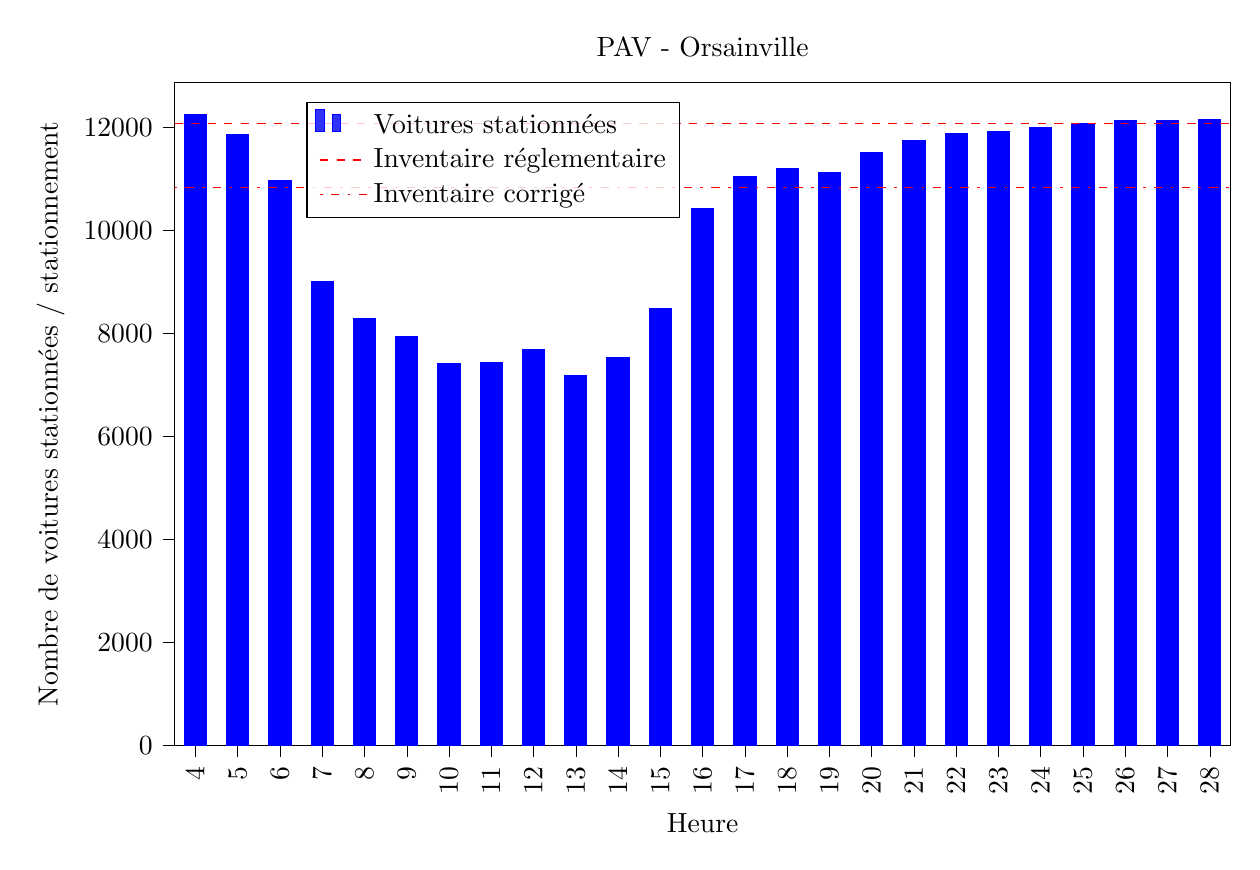
\begin{tikzpicture}

\begin{axis}[
height=10cm,
legend cell align={left},
legend style={
  fill opacity=0.8,
  draw opacity=1,
  text opacity=1,
  at={(0.125,0.97)},
  anchor=north west
},
minor xtick={},
minor ytick={},
tick align=outside,
tick pos=left,
title={PAV - Orsainville},
width=15cm,
xlabel={Heure },
xmin=3.5, xmax=28.5,
xtick style={color=black},
xtick={0,1,2,3,4,5,6,7,8,9,10,11,12,13,14,15,16,17,18,19,20,21,22,23,24,25,26,27,28},
xticklabel style={rotate=90.0},
ylabel={Nombre de voitures stationnées / stationnement},
ymin=0, ymax=12867.75,
ytick style={color=black},
ytick={0,2000,4000,6000,8000,10000,12000,14000},
yticklabels={
  \(\displaystyle {0}\),
  \(\displaystyle {2000}\),
  \(\displaystyle {4000}\),
  \(\displaystyle {6000}\),
  \(\displaystyle {8000}\),
  \(\displaystyle {10000}\),
  \(\displaystyle {12000}\),
  \(\displaystyle {14000}\)
},
scaled ticks=false
]

\addplot[ybar,draw=blue,fill=blue,legend image post style={/pgfplots/ybar legend},
  bar width=8pt]
        coordinates{
            (4,12252)
            (5,11866)
            (6,10973)
            (7,9005)
            (8,8285)
            (9,7938)
            (10,7418)
            (11,7431)
            (12,7689)
            (13,7180)
            (14,7524)
            (15,8472)
            (16,10414)
            (17,11048)
            (18,11189)
            (19,11125)
            (20,11506)
            (21,11733)
            (22,11878)
            (23,11913)
            (24,11988)
            (25,12070)
            (26,12120)
            (27,12120)
            (28,12141)
    };
\addlegendentry{Voitures stationnées}
\addplot [semithick, red, dashed]
table {%
3.5 12074
28.5 12074
};
\addlegendentry{Inventaire réglementaire}
\addplot [semithick, red, dash pattern=on 1pt off 3pt on 3pt off 3pt]
table {%
3.5 10826
28.5 10826
};
\addlegendentry{Inventaire corrigé}
\end{axis}

\end{tikzpicture}

\end{document}